\documentclass[conference]{IEEEtran}
\usepackage{bm}
\usepackage{setspace}
\usepackage{cite}
\usepackage{amsthm}
\usepackage{epsfig}
\usepackage{amsmath}
\usepackage{amssymb}
\usepackage{latexsym}
\usepackage{enumitem}
%\usepackage{enumerate}   
\usepackage{mathtools}
\usepackage{amsfonts}
%\usepackage{dsfont}
\usepackage{color}
\usepackage{optidef}
\usepackage{lettrine}
\usepackage{graphicx}
\usepackage{multicol,flushend,color}
\usepackage{wasysym}
\usepackage{float}
\usepackage{algorithm}
\usepackage[noend]{algpseudocode}
\usepackage{xcolor}
\usepackage{cuted}
%\usepackage{stfloats} 
\usepackage{url}
%%%%%%%%%%%%%%%%%%%%%%%%
%\usepackage{floatrow}
\usepackage[font=footnotesize]{caption}
\usepackage[font=footnotesize]{subcaption}


\DeclarePairedDelimiter{\ceil}{\lceil}{\rceil}
\DeclarePairedDelimiter{\floor}{\lfloor}{\rfloor}
\newtheorem{proposition}{Proposition}
\newtheorem{lemma}{Lemma}

\newcommand{\E}{\ensuremath{\mathbb E}}
\def \treq {\stackrel{\tiny \Delta}{=}}



\begin{document}
	\title{Secure Deep-JSCC
	Against Multiple Eavesdroppers}
	%{Shell \MakeLowercase{\textit{et al.}}: Bare Demo of IEEEtran.cls for Journals}		 
	
	\author{%
		\IEEEauthorblockN{%
			Seyyed 
			Amirhossein Ameli Kalkhoran$^\ast$\IEEEauthorrefmark{2}, 
			%\textsuperscript{\textsection}
			Mehdi Letafati$^\ast$\IEEEauthorrefmark{3},
			%\textsuperscript{\textsection}
			Ecenaz Erdemir\IEEEauthorrefmark{4}, 
			Babak Hossein Khalaj\IEEEauthorrefmark{3}, \\
		    Hamid Behroozi\IEEEauthorrefmark{3},  
			 and 
		Deniz G\"{u}nd\"{u}z\IEEEauthorrefmark{4}%
		}% 
\\
		\IEEEauthorblockA{\IEEEauthorrefmark{3}  \small Electrical Engineering Department, Sharif University of Technology, Tehran, Iran}%
		\IEEEauthorblockA{\IEEEauthorrefmark{2} \small Computer Engineering Department, Sharif University of Technology, Tehran, Iran}%
		\IEEEauthorblockA{\IEEEauthorrefmark{4} \small Department of Electrical and Electronic Engineering, Imperial College London, UK}%
\IEEEauthorblockA{\small Emails:‌ $\ddagger$$\{$mletafati@ee., 
			behroozi@, 	khalaj@$\}$sharif.edu;  $\dagger$ameli@ce.sharif.edu; $\S$\{e.erdemir17, d.gunduz\}@imperial.ac.uk}
}
	
	\maketitle
	\def\thefootnote{*}\footnotetext{Equal contribution}\def\thefootnote{\arabic{footnote}}
%\begingroup\renewcommand\thefootnote{\textsection}
%\footnotetext{Equal contribution}
%\endgroup
	 
	
	\IEEEaftertitletext{\vspace{-2.5\baselineskip}}
	
	
	\begin{abstract}  
% Deep learning-aided joint source channel coding  design, known as Deep-JSCC, has received significant attention in the recent years thanks to their superior performance, particularly their lack of reliance on accurate channel state information.  
% In JSCC, unlike in separable source and channel coding, the transmitted channel codeword is correlated  with the underlying source signal. While this benefits the legitimate encoder by providing robustness against channel noise, it also creates additional vulnerability in terms of leakage to eavesdroppers. 
In this paper,  a generalization of deep learning-aided joint source channel coding  (Deep-JSCC) approach to secure communications is studied.   
	We propose an end-to-end (E2E)  learning-based approach for 
		%data-driven 
		secure 
		%wireless image delivery
		communication  against
		\emph{multiple 
			%learning-assisted 
			eavesdroppers}
		over complex-valued fading channels.  
		Both scenarios of {colluding} and {non-colluding} eavesdroppers are studied.  
		For the colluding  strategy, eavesdroppers share their logits  to collaboratively infer private attributes  based on \emph{ensemble learning} method, while for   the  {non-colluding} setup  they act alone.  
		The goal 
		is to  prevent   
		%%learning-assisted
		eavesdroppers
		%adversaries 
		from inferring  private (sensitive) information about the transmitted images, while delivering  the images to a legitimate receiver with minimum distortion.  
		%Toward this end,
		%Inspired by the key idea of \emph{secrecy funnel}, 
		By generalizing the ideas of \emph{privacy funnel} and wiretap channel coding, the   trade-off between the image recovery  at the  legitimate node   
		and the information leakage to the eavesdroppers is characterized.  
		%In this paper, we assume that we do not know/have access to the data distribution, but instead have access to a dataset, and we are interested in the finite blocklength regime rather than the asymptotic limits.
		To solve  this \emph{secrecy funnel} framework,
		% we leverage  deep learning (DL)  to provide a data-driven solution.  
		% %utilize \emph{convolutional neural networks} 
		% That is, 
		we implement deep neural networks (DNNs)  
		% %comprised of convolutional layers,
		%for the communication 
		%link 
		%of legitimate parties
		to 
		%jointly
		realize a data-driven secure communication scheme, without relying on a specific data distribution.  
		%---we borrow the concept of learning-based autoencoders.  
		%Within our utilized DNN,
		%{For reconstruction at the legitimate receiver, we consider  structural similarity index 
		%(SSIM) aspect	of the  loss function during training,  to improve the perceptual quality of reconstruction.}  
		%Meanwhile,  the eavesdroppers  are also equipped with 
		%%deep learning-assisted 
		%neural decoders
%		Our 
%		%proposed approach
%		scheme   restrains  the  adversarially-trained eavesdroppers from intercepting 
%		%private information, 
%		privatized 
%		%(private/confidential)
%		data for both cases of eavesdropping a common secret,  and the case in which eavesdroppers are interested in  different secrets.
		%forestalls intercepting private information by the adversarially-trained eavesdropping nodes, 
		%such that they cannot  correctly reveal   the class  of transmitted images. 
		%to which  source  images belong.   
		%borrowing the concept of learning-based auto-encoders
		%We propose a data-driven adversarially trained deep joint source-channel coding architecture, and 
		%Moreover,  
		%Through 
		Simulations over CIFAR-10  dataset  verifies the secrecy-utility trade-off.  Adversarial accuracy of eavesdroppers are also studied over Rayleigh fading, Nakagami-$m$, and  AWGN channels to verify the \emph{generalization} of the proposed scheme.  
		%and for different communication channels, i.e., Rayleigh fading, Nakagami-$m$, and  AWGN channels.  
%		Useful insights on the \emph{secrecy-utility trade-off} 
%		%for  our  learning-based   scheme
%		are also provided.  
%		%which helps network designers maintain required parameters.   
%		%	that it is possible to
%		%	transmit to the legitimate receiver with minimal end-to-end
%		%	distortion while concealing information on the image class
%		%	from the adversary. 
Our experiments show  that  employing the proposed secure neural encoding can decrease the adversarial accuracy by $28\%$. 
	\end{abstract}
	
	
	\begin{IEEEkeywords}
	Secure Deep-JSCC, data-driven security, secrecy-utility trade-off, secure image transmission.  
	\end{IEEEkeywords}
	
	\IEEEpeerreviewmaketitle
	\vspace{-2mm}
	
	\section{Introduction} 
	\vspace{-1mm} 
	Driven by the growing interest in semantic communication systems \cite{SC},  intelligent   transmission of multimedia content
	%,  as a practical scenario of data communication, 
	has received much attention because of its various applications in  augmented/virtual reality (AR/VR),   Metaverse \cite{AdHoc}, and surveillance systems \cite{Im-retriev-deniz, caching}.      
	The adoption and success of such services rely highly on the security of the delivered contents---communication  systems  should understand the desired ``level of security'' and intelligently adapt the transmission scheme  accordingly \cite{arxive, medical}. 
	%based on contextual information  obtained  from the 6G-enabled  characteristics \cite{6G-PLS}.   
	
Connected intelligence is foreseen  as the most significant driving force in the sixth generation (6G) of wireless communications.  To this end, artificial intelligence and machine learning  (AI/ML) algorithms are envisioned to be widely  incorporated  into  6G  networks, realizing an ``AI-native'' air interface.  
Nevertheless, security issues  at the \emph{wireless edge} of 6G networks are still  identified  as  open challenges \cite{6G-PLS}. 	
	The air interface of  6G  systems encounters   ever-rising   attacks, such as eavesdropping,  spoofing  \cite{WSKG-letter},  and man-in-the-middle  \cite{WSKG-GC}.   
 

	    

	
	Recently, a considerable  number of research has been dedicated to  the utilization of deep learning (DL) techniques 
		%for encoding and decoding functions of  wireless communications.  
		to optimize the performance of  wireless  systems,
	%has emerged as a promising research direction and  
	thanks to their outstanding performance and generalization capabilities  \cite{DJSCC-Deniz,BW-agile,vtc2022}.  
	% DL-based  design 
	%is considered as a promising vision for future communication systems. 
	%%, and has gained noticeable interest.   
	In the context of  wireless security,  
	%convolutional networks \cite{BW-agile,AE-Deniz},     
 autoencoders (composed of linear layers) are exploited in  \cite{Eduard-AE}  
	%to propose a learning-based solution 
 over the additive white Gaussian noise (AWGN) wiretap channel.  
	To tackle the trade-off between the data rate and security, 
	%while achieving low error rates, scalarization approach was utilized  in terms of minimizing
	a  weighted sum of block error rate and information leakage is used as the loss function (LF) for neural wiretap code design.   
	%was minimized through training the proposed autoencoder.  
%	Simulation results show that 
%	%well-approximated
%	approximately the same performance can be achieved compared with  conventional approaches.  
	%of wiretap codes design.   
	%the drawback of their proposed model is that 
	The data fed into the autoencoder is combined with additional  non-informative random bits 
	%utilized
	to 
	%mimic 
	confuse the eavesdropper; while, this  also   reduces the communication  
	%throughput.   
	rate.   
	%the found codewords from the encoder output at Alice and the
	%noise variance of the wiretap channel are used to deal with the leakage. 
Notably, most of the previous works, i.e., \cite{MI-estim-channel_coding,MI-Wiretap-estim, Eduard-AE},   focus on  learning-aided secure channel coding, rather than  
	%proposing an E2E approach  to realize secure data-driven learning-based communication frmaework.  
	%investigating 
	taking into account the end-to-end (E2E) performance of  secure communications.  
	%	schemes 
	%	%   maintain  an undifferentiated  approach regarding
	%	ignore the source of the  bit-streams that are to be transmitted securely. 
	%%when  opting for handling   data security, 
	%rather than addressing the security for 
	%%a certain level of importancy for some 
	%sensitive (confidential/private) features of data.  
	%%being transmitted.   
	%%%%%%%%%%%%%%%%%%%%%%%%%%%%%%%%%%%%%%%%%%%%%%%
	%Moreover, except the recent works of \cite{AE-Deniz} and \cite{Ecenaz-icassp}, in the previous works  \cite{Geoff,MI-estim-channel_coding,MI-Wiretap-estim,Eduard-AE}, 
	 The content of the transmitted data is not addressed in these works and the entire bit-stream  is equally treated as the secret information to be protected against an eavesdropper.  
	%%%%%%%%%%%%%%%%%%%%%%%%%%%%%%%%%%%%%%%%%%%%%%%% 
%	In addition, none of the aforementioned works have proposed E2E learning-based  secure  communication schemes against  
%	%adversarial attacks of 
%	\emph{multiple malicious nodes equipped with adversarial neural networks}. 
%	That is, they model the 
%	%adversarial
%	attack by invoking a single exemplary Eve, and do not  investigate  the performance of their proposed schemes against multiple attackers. 
	
The E2E communication of images from a source node  to a legitimate destination  can be considered as  a joint source channel coding (JSCC) problem. DL-aided JSCC design, a.k.a  Deep-JSCC, has received significant attention thanks to its  superior performance, particularly its lack of reliance on accurate channel state information \cite{DJSCC-Deniz}.  
	However, in JSCC, different from  separate   source and channel coding, the channel codeword is correlated  with the underlying source signal.  This can create vulnerabilities  in terms of leakage to eavesdroppers, despite  providing robustness against channel noise. 
	%We also note that classical encryption methods are not applicable here as they would destroy the correlation between the source and the channel input.  
	Inspired by \cite{AE-Deniz} and \cite{Ecenaz-icassp}, we provide a generalization of the Deep-JSCC approach   to secure communication problems against multiple eavesdroppers.
		% by formulating a secrecy funnel framework  \cite{funnel}. 
		%The DNN-based design of JSCC in \cite{AE-Deniz,Ecenaz-icassp} is particularly attractive for the design of secure content delivery schemes, since they can learn the security sensitivity of different parts of the contents, and adopt their transmission strategy  accordingly.   
		In this regard, \cite{AE-Deniz} proposes  a generative adversarial network (GAN)-inspired secure neural encoder-decoder pair  over an AWGN wiretap  channel  against one eavesdropper.   The authors in \cite{Ecenaz-icassp}  propose  a variational autoencoder (VAE)-based approach for Deep-JSSC design  over binary symmetric channels, again considering  a single eavesdropper.  
		%However, none of them considered the secure communication over against  
		
		In this paper, we consider  \emph{E2E learning-based   secure communication  against  multiple eavesdroppers} for both colluding and non-colluding eavesdroppers,  over AWGN as well as  fading channels.  
For the  scenario of colluding  eavesdroppers, the adversaries share their logits to collaboratively infer private attributes based on  the \textit{ensemble learning} approach, while for   the  {non-colluding} setup  they act alone.   
	Please see Fig. \ref{fig:SysModel} for an illustration of the communication scenario studied in this paper.  
		%%%%%%%%%%%%%%%%%%%%%%%%%%%%%%%%%%%%%%%%%%%%%%
	Applications of our proposed framework include  (but are not limited to) 
	%one can consider 
	digital healthcare services, in which medical images   are sent to or received from  access points, while some private attributes, e.g., the identity of  patients should be kept  secret from potential eavesdroppers.  
	%%%%%%%%%%%%%%%%%%%%%%%%%%%%%%%%%%%%%%%%%%         
	%%%%%%%%%%%%%%%%%%%%%%%%%%%%%%%%%%%%%%%%%%%  
	%%%%%%%%%%%%%%%%%%%%%%%%%%%%%%%%%%%%%%%%%%%%%%%
	Notably, previous works \cite{AE-Deniz} and \cite{Ecenaz-icassp}  only considered a single eavesdropper with a single-antenna transmitter and multiple parallel channels, respectively. 
	%with one exemplary Eve. 
	In addition, both  \cite{AE-Deniz} and \cite{Ecenaz-icassp} are limited to static channels.  
	Moreover,  different from \cite{Eduard-AE}, no additional 
	%random 
	redundant bits are required to be added to the source image.  
	%  To elaborate, our proposed approach restrains  adversarially-trained eavesdropping nodes from intercepting private information,  in a way  that they cannot  correctly infer  certain sensitive attributes. 
{In this paper, Rayleigh fading channel model is used  to represent time-varying  channel realizations during training, while  inference is performed over Nakagami-$m$ and AWGN channels, %(well-established  models for time-varying wireless  channels), 
in addition to Rayleigh fading. 
Note that the encoder and the decoder  do not require any knowledge of the instantaneous channel gains in the proposed scheme.}	\footnote{\textit{Notations:} We denote the transpose, the conjugate transpose,  and $\ell^2$ norm of a vector by $(\cdot)^\mathsf{T}$, $(\cdot)^\dagger$,  and $||\cdot||$, respectively. 
%		Moreover, $|\cdot|$ represents
%		the absolute value of a scalar variable and 
%		%$\mathrm{card}(\cdot)$ denotes
%		the cardinality of a set.    
%while matrices are written  as bold uppercase symbols.      
The expected value and the probability density function (pdf) 
%the cumulative distribution function (CDF), and the complementary cumulative distribution function (CCDF) 
of random variable (RV) ${X}$ are denoted by $\E[{X}]$ and $p_X(x)$, 
%$F_X(x)$, and $\overline{F}_X(x)$, 
respectively.  
Realization vectors of RVs are represented by bold lowercase letters. 
%	Moreover, the probability of an event $A$ is denoted by $\mathsf{Pr}(A)$.
The mutual information of RVs ${X}$ and ${Y}$ and the cross-entropy  of two distributions $p$ and $q$ are shown, respectively, by $I({X};{Y})$ and $H(p,q)$.  
%	We also denote $[x]^+=\max(x,0)$.  
%$(a)_n$ stands for the Pochhammer symbol.}
%Also, the operator $\circ$ indicates Hadamard (elementwise) operations.
}
 
	
	
	%%%%%%%%%%%%%%%%%% Add this to the problem %%%%%%%%%%%%%%%%  formulation part of the paper:‌
	%In addition to the SC-based techniques, the
	%more general trade-off between the communication rate and
	%the private message’s equivocation (secrecy) rate has also been addressed in [1,2,4–7].
	%Here, we consider the more general setting studied in [3], where we consider the lossy delivery of an information source to the legitimate receiver, while limiting the information leakage to  adversaries.
	%We will further generalize the model in [3: Yamamoto], and assume that the transmitter only wants to keep a certain sensitive part of the information source (S) secure from the set of eavesdroppers.  
	%Although This formulation of Yamamoto is attractive as it provides
	%theoretical and quantifiable security guarantees; however, its
	%application to practical systems is limited due to the idealistic
	%and perfectly known source and channel distributions, and the
	%result does not hold in practical finite blocklength regimes. 
	% Instead, we take into account...  the trade-off/privacy xyz between the distortion achieved at the legitimate receiver and the leakage to  eavesdroppers (adversaries) is considered in a practical non-asymptotic regime. 



	
	\begin{figure}
		\vspace{0mm}
		\centering
		\includegraphics
		%[width=3.0in,height=3.5in,trim={0.0in 0.0in 0 0.75in},clip]
		[width=3.75in,height=1.15in,trim={0.25in 0.2in 0.1in  0.35in},clip]{AE_SysMod_8.eps}
		\vspace{-5mm}\caption{Proposed system model for secure  transmission against 
			%adversarial networks
			multiple eavesdroppers.}
		\label{fig:SysModel}
  \vspace{-5mm}
	\end{figure} 
	
	
	
	
	\vspace{0mm}
	\section{System Model and Problem Statement} \label{sec:System_Model}	 
    \vspace{-1mm}
	Consider the  communication scenario  depicted  in Fig. \ref{fig:SysModel}, where a multi-antenna source  node, Alice ({$\cal A$}) with $n_{\sf T}$ antennas, aims to  deliver an image {${U}^n \in \mathcal{U}^n$}  to a  destination  node, Bob ({$\cal B$}), 
	over $k$  uses of 
	the  communication  channel, 
  {where $\mathcal{U}$ denotes the alphabet of source images.}     
	According to the JSCC literature \cite{DJSCC-Deniz}, we refer to  the image dimension, $n$,  as the  {source bandwidth}.  The channel dimension $k$  characterizes  the {channel bandwidth}, where we  usually have  $k < n$ to reflect the concept of {bandwidth compression}  \cite{DJSCC-Deniz}.   
	%Accordingly, the ratio $k/n$ stands for the  {bandwidth compression ratio}.  
	Image delivery should be kept secret from multiple eavesdroppers, denoted by Eve$_{1}$($\mathcal{E}_1$), $\cdots$,  Eve$_{M}$($\mathcal{E}_M$), which overhear the communication through 
	%wiretap 
	their own channels,  
	% and are equipped with adversarial DNNs, 
	and want  to infer a private (sensitive)  attribute, e.g., diagnostic information regarding the source image, denoted by  $S \in \mathcal{S}$ with a discrete alphabet $\mathcal{S}$. 
	%, i.e.,  
	%More specifically, the adversaries   try to figure out  
	%the class to which  the transmitted  images belong.    
{The eavesdroppers in the non-colluding setup act alone to infer the secret $S$,  
	%and  their  training is performed based on their individual LFs  given in the subsequent section.  
	while for the colluding setup,  ``knowledge sharing'' is also performed---they share  their logits based on    the concept of \emph{ensemble learning} 
	%to infer the secret $S$ 
	\cite{ensemble}.}

	
	
	\begin{figure*}
		\vspace{0mm}
		\centering
		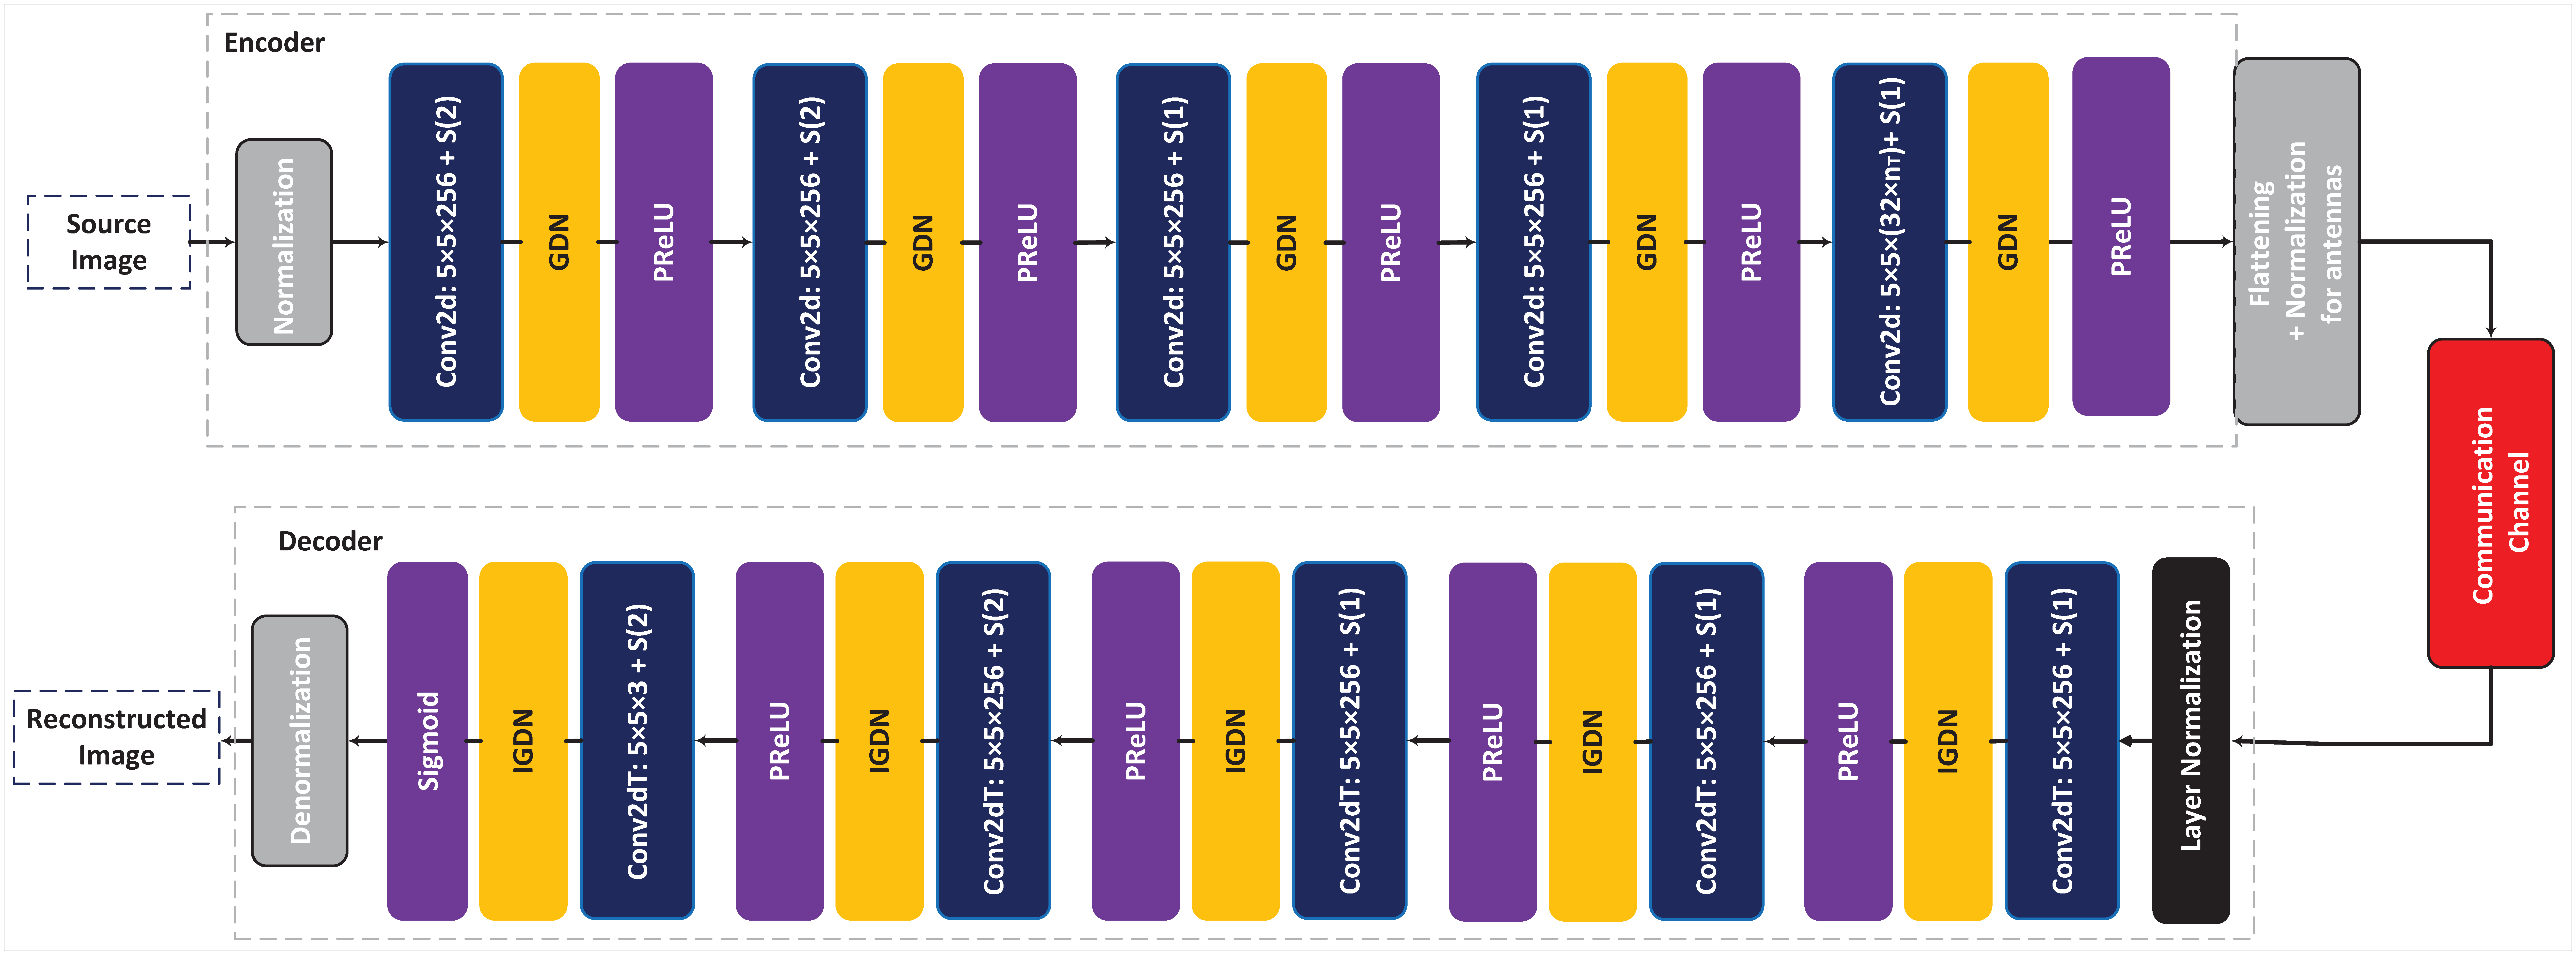
\includegraphics
		[width=5.5in,height=2in,trim={0.1in 0.1in 0.1in 0.4in},clip]{AE_SysMod_5.eps}
		\vspace{0mm}
		\caption{Proposed DNNs at Alice (encoder) and Bob (decoder). 
			The notation $w\times w \times f$  denotes a convolutional layer with $f$ filters of spatial extent 
			%(size)
			$w$. 
			%			The notation $w\times w \times (f \times n_{\sf T})$ at the last convolutional layer of encoder indicates that we require $f$
			%			%\times n_{\sf T}$ 
			%			filters for each of  $n_{\sf T}$ antennas at the  encoder output.  
			Moreover,  $s(\cdot)$ denotes  the stride, which  can be downsampling (at the encoder) or upsampling (at the decoder) \cite{DJSCC-Deniz}. At the output of the last 
			PReLU layer, which consists  of $2k \times n_{\sf T}$ elements, 
			%of encoder DNN, 
			we employ a flattening layer for each of the $n_{\sf T}$ antennas,  to reshape the  encoded tensor  to a data-stream.   The encoded latent sequence is further  normalized, such that the channel input satisfies the average transmit power constraint. }
		\vspace{-5mm}
		\label{fig:DNN}
	\end{figure*} 
	
	
	%%Considering  the E2E  image transmission over  wireless communication channel,  
	%The image data \textcolor{blue}{${U}^n \in \mathcal{U}$}  should be delivered  from Alice to Bob  over $k$  uses of the  communication channel, \textcolor{blue}{where $\mathcal{U}$ denotes the alphabet of source images.}  
	%According to the JSCC literature \cite{DJSCC-Deniz}, we refer to  the image dimension, $n$,  as the  {source bandwidth}.  The channel dimension $k$  characterizes  the {channel bandwidth}, where it usually holds that $k < n$,  which reflects the concept of {bandwidth compression}.  (Please see \cite{DJSCC-Deniz} and references therein for more details.)  
	%%Accordingly, the ratio $k/n$ stands for the  {bandwidth compression ratio}.  
	%The  signals transmitted over the air  are  also overheard by adversaries in a noisy manner.  
	%who receive  a noisy version of the data. 
	%Specifically, 
 
% \vspace{0mm}
% As shown in Fig. \ref{fig:SysModel}, Alice aims to  reveal $U^n$ to Bob  with minimum distortion, 
%	%under a given distortion measure $d(\cdot, \cdot)$, 
%	while preventing the   information of  sensitive  part 
%  {$S$}  to be leaked to any of $M$  eavesdroppers. 
%  %, $i = 1,\cdots,M$, where  $M$ denotes the number of eavesdroppers. 
%The sensitive (private) parts are   correlated with $U^n$  with distribution  $p_{U^n,S}$.  
	Alice  maps the source information 
	%encodes
	%Alice  maps  each realization of  the source information  $U^n$  denoted by  $\bm  u \in \mathbb{R}^n$,   to a vector of   channel input $X^k$.   ${\bm x} \in \mathbb{C}^k$. 
	$U^n$ into a {channel input codeword $X^k \in \mathbb{C}^{n_{\sf T} \times k}$} via an encoding 
	function {$f_{\cal A}: \mathcal{U}^n \rightarrow \mathcal{X}^k$}, where  $X^k = f_{\cal A}(U^n)$.  
	%Considering the practical scenarios in real-world communications, networks  are faced with  limited energy; thus,  
	%%is required to 
	%one should satisfy 
	Transmitted codeword is subject to an average
	power constraint, $\frac{1}{k} \mathbb{E}[({X^k})^\dagger{X^k}] \leq P$, which will be satisfied for the realizations of the channel codeword in our data-driven approach.
	%Note that, we assume that A does not directly observe S. 
	%%%%%%%%%%%%%%%%
	%	The 
	%%output at  Alice's  transmitter
	%	encoded data-stream  $X^k$ is sent  over the communication  channel.   
	%%$\eta_{h_i}(\cdot)$ for $h_i \in$ $\cal A$-to-$\cal B$ and $\cal A$-to-Adversaries links.   
	%%%%%%%%%%%%%%%%	
	Channel outputs at $\mathcal{B}$ and $\mathcal{E}_m$  are denoted, respectively, by $Y^k$ and $Z_m^k \in \mathbb{C}^k$, with $m \in \{1, \ldots, M\}$.  
	%which is characterized by the joint conditional distribution 
	%In other words, we have $Y^k = \eta^{\sf leg}(X^k)$ and $Z^k_i = \eta^{\sf adv}_i(X^k) $, where $\eta^{\sf leg}$ and...  	
	Transmission of data-streams over the air  experiences  independent realizations of the  conditional   channel distribution $p_{Y, Z_1, \ldots, Z_M |‌X  }$.    
	We consider both the AWGN and  slow fading channels, where for the slow fading, we adopt two widely-used models of Rayleigh fading and Nakagami-$m$ channels, and {assume the channel realization to remain constant for the duration of the transmission of a single image, i.e., for $k$ channel uses.}
	Bob then applies a  decoding function
	$f_{\cal B}$ to obtain $\hat{U}^n = f_{\cal B}(Y^k)$. 
	Meanwhile, each Eve tries to extract the sensitive attribute  $S$, from her observations $Z_m^k$, or by collaborating with other Eves, i.e., sharing their logits. 
	%Denoting $Z_i^k$ as the observation (the received signal) of the $i$'th adversary,  
	We consider the trade-off between  delivering images
	%$U^n$ 
	to Bob with the highest fidelity and  controlling  the information leakage to each adversary, which  
	%% in a way that the  sensitive/private  part ($S$) of the information source should be kept secret from the adversarial nodes.  
	%The   information leakage to each of the  adversaries  
	is theoretically 
	measured	by the mutual information metric  $I({S};{ Z}_m^k)$. 
%	Fundamentally,  the  trade-off between the minimum  achievable distortion at the  legitimate receiver and the minimum  leakage to Eve is asymptotically   characterized  in \cite{Yamamoto} under the idealistic assumption of i.i.d. source and channels with known distributions, which are not  applicable  to practical systems 
%	with finite block-lengths 	and unknown source and channel statistics.
%	In our system model 
%	%we consider a \emph{data-driven} approach for the  practical non-asymptotic regime. That is,  
%	we do not consider  any underlying  assumption on the distribution of the data source  or the latent private variable.  
%	%Instead,   we have  access to  datasets to facilitate the process of learning optimized secure encoding-decoding pairs.
Inspired by the key idea of \emph{privacy funnel} \cite{funnel},  we first formulate  an optimization   framework to characterize  this trade-off,  which we call \emph{secrecy funnel}. 
	This funnel-like framework is then  solved in a data-driven manner by implementing   DNNs.  
	Mathematically, we aim to simultaneously minimize both the distortion $d(U^n,\hat{U}^n)$ at Bob and the information leakage,  $I({S};{ Z}_m^k), m \in [M]$ to adversaries. 
	This corresponds to the following problem 
	%as  a weighted sum  of the multiple objectives with  weights $w_m \in \mathbb{R}_{>0}$ as follows:‌ 
	\begin{align}\label{eq:P0}
		\underset{
			f_{\cal A},
			f_{\cal B}}{\text{minimize}}
		\quad 
		\mathbb{E}\left[d(U^n,\hat{U}^n)\right] + 
		%\underset{i\in\{1,\cdots, M\}}{\text{max}}
		\frac{1}{M}	\hspace{0mm}  \sum_{m \in [M]} w_m I({S};{ Z}_m^k),   
	\end{align}
where $w_m$  shapes our secrecy funnel and   adjusts the trade-off between  the information leakage and the distortion.     
%	To  make  \eqref{eq:P0} tractable, 
%	%the challenge is 
%	we   further need to estimate the mutual information term in our problem.   
%For this, we   apply the variational 
%	%lower bound 
%	approximation  proposed in \cite{MI-approx} for  the mutual information metric and obtain
Numerical solution of optimization \eqref{eq:P0}   is intractable due to the mutual information term.  Hence, we apply a variational approximation of mutual information, which was proposed in \cite{MI-approx}. Then, our optimization can be rewritten as:‌ 
	\begin{align}\label{eq:P1}
		\underset{f_{\Omega_{\cal A}},
			f_{\Omega_{\cal B}}}{\text{minimize}} \quad  \hspace{-2.5mm}\mathbb{E}\hspace{-0.5mm}\left[\hspace{-0.3mm}d(U^n,\hat{U}^n)\hspace{-0.3mm}\right] \hspace{-1mm} + \hspace{-1mm}‌
		\frac{1}{M}	\hspace{-2.5mm} \sum_{m \in [M]}  \hspace{-3mm}
		w_m
		\underset{q_{S|Z_m^k}}{\text{max}}\hspace{0mm}
		\hspace{-1mm}\mathbb{E}\hspace{-0.5mm}\left[\log q_{S|Z^{k}_{m}}(s|{\boldsymbol z}_m)\hspace{-0.5mm}\right],  
	\end{align} 
	%secrecy and distortion.   	
	where $q_{S|Z^k_m}(s|{\boldsymbol z}_m)$ characterizes the  
	Eve$_{m}$'s posterior  estimation corresponding to the correct
	distribution of $S$, 
	%estimated  distribution of $S$ at the adversary 
	given the observation $Z^k_m = {\boldsymbol z}_m$. 	
To realize a data-driven approach,  $f_{\cal A}$ and $f_{\cal B}$ are parameterized by DNNs with parameters $\Omega_{\cal A}$ and $\Omega_{\cal B}$, respectively.  
Details of the DNN architectures and the  training strategies  are given in the next section.     
	The approximation  in \eqref{eq:P1} can be interpreted as the sample-wise negative  cross-entropy (CE)  between the distribution over  adversaries' predictions and the true 
	%conditional 
	distribution of sensitive attributes. 
	To solve \eqref{eq:P1} in a data-driven manner, we assume that the 
	% assuming  any  knowledge about the underlying distribution of  image source and the private  attributes, we  implement  DNNs to employ the secure  encoding-decoding functionalities  at $\cal A$ and $\cal B$, while the 
	Eves also employ  adversarially-trained DNNs and try  to infer the sensitive attributes of the transmitted images, where  
	%Let $\Omega_{\cal A}$ and $\Omega_{\cal B}$  stand for the set of (trainable) parameters of the encoder and decoder pair at Alice and Bob, respectively. 
	%In addition, let 
	$\Theta_{E,m}$  parameterizes  the adversarial network of Eve$_{m}$. 
	Accordingly, we can formulate the following  LF.   
	%by the DNN counterparts. 
	\begin{align}\label{eq:P-DL}
		\hspace{-2mm} \mathcal{L}(\Omega_{\cal A},\Omega_{\cal B},&\mathbf{\Theta}_E)     = 
	   \mathbb{E}\left[d(U^n,f_{\Omega_{\cal B}}(Y^k))\right]  \nonumber
		 \\ 
		& + 
		%\underset{i\in\{1,\cdots, M\}}{\text{max}}
		%\quad 	
		\frac{1}{M}	\hspace{0mm} \sum_{i \in [M]} w_m \hspace{2mm} \underset{\Theta_{E,m}}{\text{max}}
		\hspace{1mm}
		\mathbb{E}\left[\log q_{\Theta_{E,m}}({s|{\boldsymbol z}_m})\right],  
	\end{align}
	where  $\mathbf{\Theta}_E \overset{\Delta}{=} (\Theta_{E,1}, \cdots,\Theta_{E,M})$, 
	%$f_{\Omega_{\cal A}}$ and $f_{\Omega_{\cal B}}$  represent  the encoder and decoder functionality of Alice and Bob's DNNs, respectively,   for which we have   $X^k = f_{\Omega_{\cal A}}(U^n)$. 
	%Moreover, 
	and $q_{\Theta_{E,m}}({s|{\boldsymbol z}_m})$ formulates the approximated adversarial   likelihood regarding  the correct value $S=s$, 
	%which is
	estimated  by the DNN of the  $m$'th adversary. 
	Details of the 
	%rationality behind our
	proposed DNN architectures and the training strategies  are given in the following  section. 

	%%%%%%%%%%%%%%%%%%%%%%%%%%%%%%%%%%%%%%%%%%%%%%%%%%%%
	%    \footnote{We note that other channel models can be considered likewise.   
	%    %in a similar manner with
	%    We  merely require  the channel transfer function to be  differentiable,  allowing the gradient computation and error back-propagation steps to be performed.}   
	%	%without compromising the back-propagation step.
	%%%%%%%%%%%%%%%%%%%%%%%%%%%%%%%%%%%%%%%%%%%%%%%%%%%%%
	 
 

	
	
	
	
	\vspace{-0mm}
	\section{DNN Architectures}\label{sec:Proposed_approach}
	\vspace{-0mm}
	According to the Deep-JSCC concept \cite{DJSCC-Deniz}, 
	we employ  autoencoder DNNs  to  directly map the  image pixels to  channel input symbols. 
	%To elaborate, 
%	Consider image input files with dimensions $n = H \times W \times C$, where $H$, $W$, and  $C$ stand for the image height, width,  and  the number of channels ($3$ for colored images and $1$ for grayscale), respectively. 
	In  this regard, $\cal A$ maps  each realization of  the source data  $U^n$,  denoted by  $\bm  u \in \mathbb{R}^n$,   to a vector of   channel input   ${\bm x} \in \mathbb{C}^k$, which can be viewed as a realization of  $X^k$.  
	%Following the  JSCC scheme, that bypasses the transformation of the pixel values to a sequence of bits, which are then mapped again to complex-valued channel inputs; and instead, directly maps the pixel values to channel inputs as in \cite{SoftCast:Allerton:10, Tung:CL:18}.
	The block diagram of the DNNs employed for  the neural encoder and decoder components of  legitimate parties  is illustrated in Fig. \ref{fig:DNN}. 
	In addition, the DNN structure employed by each of the  adversaries is demonstrated in Fig. \ref{fig:DNN-Advs}. 
	%\footnote{We state that the  considered  hyper-parameters for the  legitimate DNNs, as demonstrated in Fig. \ref{fig:DNN}, are  selected  based on  comprehensive  experiments and numerous trials, while the
	%	%main concept for a
	%	general architecture is inspired by \cite{Deniz-GDN}.}  
		
	\begin{figure}
		\vspace{-3mm}
		\centering
		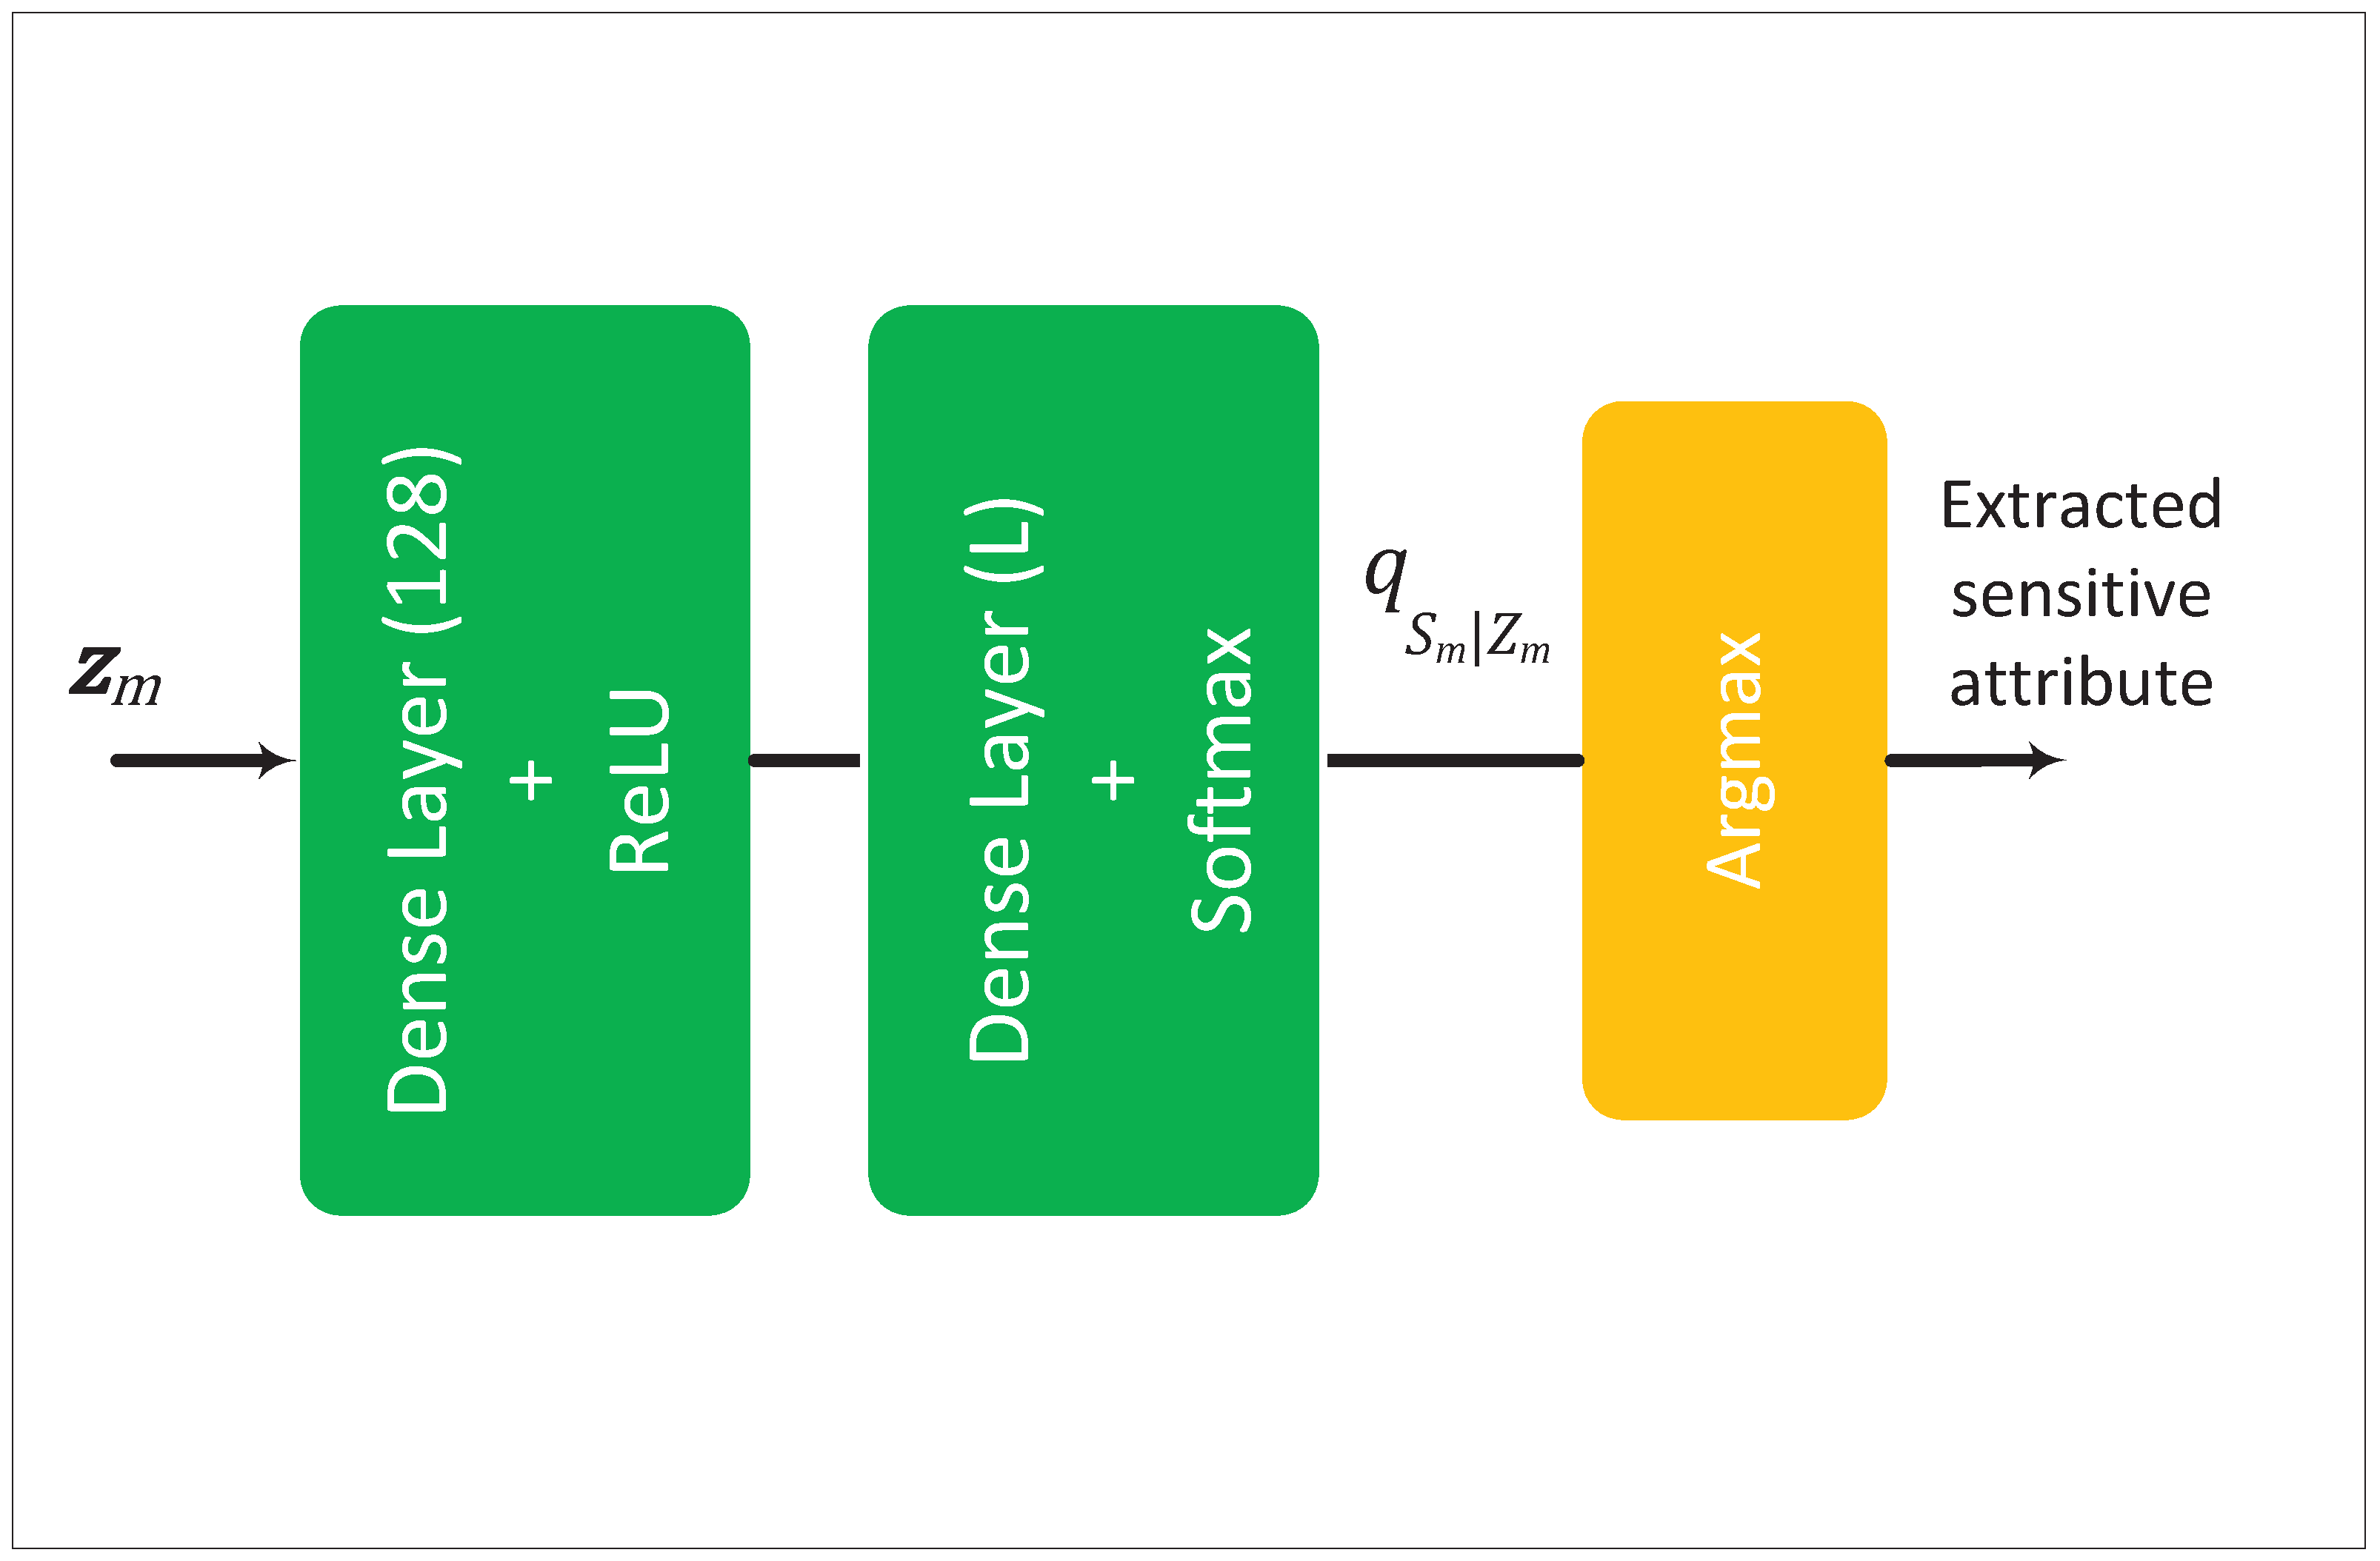
\includegraphics
		[width=2.85in,height=1.65in,
		trim={0.1in 1.75in 0.1in 1.0in},clip]{AE_SysMod_6.eps}
		\vspace{-3mm}
		\caption{Implemented DNN at adversaries for extracting sensitive information.}
		\label{fig:DNN-Advs}
  \vspace{-4mm}
	\end{figure} 
\vspace{0mm}


	%The structure of  adversarial DNNs, which are parameterized by $\Theta_{E,i}, i \in [M]$,   is presented  in Fig. \ref{fig:DNN-Advs}.
\vspace{-0.5mm}	
According to the proposed system model,  adversaries 
	%main reason of 
	utilize DNNs to facilitate the inference   of  sensitive  information $S$ from their received signals.  $S$ can be 
	%assumed to be 
	the class labels of the images  \cite{AE-Deniz, Ecenaz-icassp}.    
	For example, the identity of patients within  medical imaging in e-health applications.    
	To 
	% this goal,
	infer   sensitive attributes from images,  each adversary employs the DNN architecture illustrated in Fig. \ref{fig:DNN-Advs}, where the  dimension of the  output  neurons, $L$, equals the 
	%  number of classes $L$
	cardinality  of the secrets $|S|$.\footnote{It would be interesting to 	study the  performance when the eavesdroppers employ more complicated neural  architectures, such as VGG and ResNet variation, to infer the secret. This will be addressed in our future works.} 
	The output of the softmax layer produces  an adversarial likelihood  estimation regarding the posterior  distribution  $q_{\Theta_{E,m}}({s_m|{\boldsymbol z}_m})$.  
%	$\forall m \in [M]$. 
	\vspace{-0.5mm}
	Invoking  \eqref{eq:P-DL},  one can say that each Eve  tries to minimize its CE between the adversarially-estimated posterior  distribution $q_{\Theta_{E,m}}({s_m|{\boldsymbol z}_m})$ and the ground-truth, which is represented by the one-hot encoded vector of $S$, denoted by  $ {{\bm \varepsilon}_s} \in \{0,1\}^L$.   
	Notably, having lower CE values results in  
	%i.e.,
	higher similarity between the  adversarial posterior distribution    	and the ground-truth, which increases the information leakage in terms of CE.    
	Meanwhile, $\cal A$ and $\cal B$  try to jointly  minimize the reconstruction distortion  and the information leakage  measured by the negative CE metric. 
Hence,  the  sample-wise  communication framework  can be reformulated as:   
	\begin{align}\label{eq:P-DL-CE}
		\text{minimize}	\hspace{2mm} & \mathcal{L}(\Omega_{\cal A},\Omega_{\cal B},\mathbf{\Theta}_E)  = 
		\mathbb{E}_{p(\bm{u},\bm{\hat{u}})} \left[	d\left(\bm u,
		%f_{\Omega_{\cal B}}(\bm y)
		\bm{\hat{u}}
		\right)
		\right] 
		\nonumber \\ 
		& \hspace{-2mm}+ 
		%\underset{i\in[1:M]}{\text{max}}
		%\quad 	
		\frac{1}{M}	\hspace{-2mm} \sum_{m \in [M]} \hspace{-2mm}  w_m \hspace{1mm}
		\underset{\Theta_{E,m}}{\text{max}}
		\hspace{0.5mm}
		%\mathbb{E}\left[
		%	\log q_{\Theta_{E,i}}({s|z_i})
		\left(- H\hspace{-1mm}\left(q_{\Theta_{E,m}}({s|{\boldsymbol z}_m}),{{\bm \varepsilon}_s}\right)\right), 
		%\right]  
	\end{align}
	where $\hat{\bm u} = f_{\Omega_{\cal B}}(\bm y)$, and 
	$p(\bm u, \hat{\bm u})$ stands for the joint probability distribution of the original and the reconstructed image, taking into account the randomness in the input image and the channel. 
	Since  the true distribution $p(\bm u)$ is often unknown, we estimate the expected distortion measure  using samples ${\bm u}_j$ from an available  dataset ${\cal D}_u$ by computing $\mathbb{E}_{p(\bm{u},\bm{\hat{u}})} \left[	d\left(\bm u,f_{\Omega_{\cal B}}(\bm y)\right)
	\right] \approx \frac{1}{N_u}\sum_{\bm{u}\in \mathcal{D}_u} d(\bm u, \hat{\bm u})$, where  
	%is the training dataset, and
	 ${N_{u}} \overset{\Delta}{=} |\mathcal{D}_u|$.
	 % denotes its cardinality.  	
	{It is assumed  that we know the sensitive attribute in which the eavesdroppers are interested, as well as their channel models.  Both of these assumptions  are common  in the privacy \cite{AE-Deniz, Ecenaz-icassp} and wiretap channel \cite{Eduard-AE,  MI-Wiretap-estim, MI-estim-channel_coding} literature.  
	%	We also remark that 
	We do not need to know the instantaneous channel gains, but use their distributions to sample channel realizations during training.}     
	
	\vspace{0mm}
	\subsubsection*{Training Procedure}\label{sec:training}
	In order to train our  system  based on   \eqref{eq:P-DL-CE}, we  follow an  iterative procedure.  
	Intuitively, the network nodes  are faced  with a  minimax game, i.e., the competition between legitimate autoencoder and the adversarial  DNNs.  
	%To solve the minimax game, i.e., the competition between legitimate autoencoder network and the adversarially-trained  networks,
	%we can provide the following discussion. 
	Hence,  the following strategy is run  through our proposed E2E system:  	
		The encoder and decoder function of Alice and Bob should jointly minimize their LF, denoted by $\mathcal{L}_{\cal AB}$:  
		% $\mathcal{L}_{\cal AB}$ given below  
        \begin{align}
        & \hspace{0.5mm}\mathcal{L}_{\cal AB}  =
         \nonumber \\
         &  \hspace{0.5mm} \frac{1}{N_{u}}\hspace{-1.5mm}\sum_{{\bm u} \in \mathcal{D}_u}
			\hspace{-1.5mm} \left( \hspace{-1mm}
			d(\bm u, \hat{\bm u})\hspace{-1mm}-
			\hspace{-1mm}\frac{1}{M} \hspace{-2mm}\sum_{m \in [M]} \hspace{-3mm} w_m \hspace{0mm}
		H\hspace{-0.5mm}\left(\hspace{-0.5mm}q_{\Theta_{E,m}}\left({s{(\bm u)}|{\bm z}_m{(\bm u)}}\right),{{\bm \varepsilon}_{s}}{(\bm u)} \hspace{-0.5mm} \right)\hspace{-1.9mm}
			\right)\label{eq:L_AB}
        \end{align}
	% 	\begin{figure*}[!t]
	% 		\vspace{-5mm}
	% 		\centering    	
	% 	\begin{align}\label{eq:L_AB}
	% 		%	\mathcal{L}_{\cal AB} = \mathbb{E}_{p(\bm{u},\bm{\hat{u}})} \left[	d\left(\bm u,f_{\Omega_{\cal B}}(\bm y)\right)
	% 		%	\right]
	% 		%	- ‌w\underset{i\in[1:M]}{\text{max}}
	% 		%	%\quad 	
	% 		%	\hspace{1mm}
	% 		%	\underset{\Theta_{E,i}}{\text{max}}
	% 		%	\hspace{0.5mm}
	% 		%	%\mathbb{E}\left[
	% 		%	%	\log q_{\Theta_{E,i}}({s|z_i})
	% 		%	H\hspace{-1mm}\left(q_{\Theta_{E,i}}({s|z_i}),\bm \varepsilon_s\right)
	% 		\mathcal{L}_{\cal AB} & =  \frac{1}{N_{\cal T}}\sum_{j=1}^{N_{\cal T}}
	% 		\left(
	% 		d(\bm u_j, \hat{\bm u_j})
	% 		- 
	% 		% \underset{i\in[1:M]}{\text{max}}
	% 		%\quad 	
	% 		\hspace{1.5mm}
	% 		%\mathbb{E}\left[
	% 		%	\log q_{\Theta_{E,i}}({s|z_i})
	% 		\frac{1}{M} \sum_{i \in [M]}  w_i \hspace{0mm}
	% 		H\hspace{-1mm}\left(q_{\Theta_{E,i}}({s^{(j)}_i|z^{(j)}_i}),{{\bm \varepsilon}_{s}}^{(j)}_i\right)
	% 		\right). 
	% 		\\
	% %\end{align} 
	% %\hrulefill
	% %\begin{align}
	% 	\mathcal{L}^{\sf ALC}_{\cal AB} & =  \frac{1}{N_{\cal T}}
	% 	\sum_{j=1}^{N_{\cal T}}
	% 	\left(
	% 	d({\bm u_j}, {\hat{\bm u}}_j)
	% 	+  \hspace{0mm}
	% 	%\underset{i\in[1:M]}{\text{max}}
	% 	%\quad 	
	% 	%\mathbb{E}\left[
	% 	%	\log q_{\Theta_{E,i}}({s|z_i})
	% 	\frac{1}{M} \hspace{0mm} \sum_{i \in [M]}  w_i 
	% 	H\hspace{-1mm}\left(q_{\Theta_{E,i}}({s^{(j)}_i|z^{(j)}_i}),\bar{p}_L\right)
	% 	\right). 	\label{eq:L_AB-LE}
	% \end{align}
	% \hrulefill
	% \end{figure*}
		%Before going through the details of the training process, 
	%We take one further step within  
	The training process of legitimate nodes can be further enhanced via employing  \emph{adversarial likelihood compensation} (ALC), which has been shown in \cite{AE-Deniz} to be more effective in confusing an adversary than the one-hot encoding approach.   
		The main idea is to make the posterior distribution  of  adversaries 
		%look
		%mimic
		imitate a uniform distribution $\bar{p}_L = [\frac{1}{L},\cdots,\frac{1}{L}]^{\sf T}$. 
		%in order to 
		Hence, {Alice and Bob jointly maximize the uncertainty of adversarial  predictions, resulting in 
		the following  loss function 
        \begin{align}
         & \hspace{0.5mm} \mathcal{L}^{\sf ALC}_{\cal AB} \hspace{-0.5mm}  = \nonumber \\
         & \hspace{0.5mm} \frac{1}{N_{u}}\hspace{-1mm}
		\sum_{{\bm u} \in \mathcal{D}_u} \hspace{-2mm}
		\left( \hspace{-1mm}
		d({\bm u}, {\hat{\bm u}}) \hspace{-1mm}
		+  \hspace{-1mm}
		\frac{1}{M} \hspace{-1.5mm} \sum_{m \in [M]} \hspace{-1.5mm} w_m
		H\hspace{-0.5mm}\left(q_{\Theta_{E,m}}({s{(\bm u)}|{\bm z}_m{(\bm u)}}),\bar{p}_L \hspace{-0.5mm}\right)\hspace{-1.0mm}
		\right) \label{eq:L_AB-LE}
        \end{align}
    	The distortion measure we consider for our legitimate loss function $	\mathcal{L}_{\cal AB}$ is a mixture of the average mean squared error (MSE), denoted by ${\Delta}^{\sf{MSE}}$, and 
    the structural similarity index (SSIM), ${\Delta}^{\sf{SSIM}}$,  between the  input image $\bm u$  and the recovered version $\hat{\bm u}$  at the output of Bob's DNN.
    Therefore, we assume $d(\cdot,\cdot)$ to be measured  as follows 
    \begin{align}\label{eq:distortion}
    	d(\bm u , \hat{\bm u}) = 
    	%(‌1-\alpha) 
    	{\Delta}^{\sf{MSE}}(\bm u , \hat{\bm u}) + 
    	\alpha {\Delta}^{\sf{SSIM}}(\bm u , \hat{\bm u}),
    \end{align}
    where 
    %\begin{align}
    $	\Delta^{\sf MSE} (\bm u , \hat{\bm u})
    %&
    \overset{\Delta}{=}\frac{1}{n}||\bm u-\hat{\bm u} ||^2$,  
    %\nonumber \\
    %\quad  
    $\Delta^{\sf SSIM}(\bm u , \hat{\bm u}) \overset{\Delta}{=} 1- 	\mathsf{SSIM}(\bm u, \hat{\bm u}),  
    $  
    %\end{align}
    %with $n$ denoting the size of the original image  vector $\bm u \in \mathbb{R}^n$. Moreover,
    and $\alpha$ is a tuning parameter representing the contribution of the SSIM metric.  
    The SSIM measure between two images $I$ and  $K$ is defined as 
    \begin{align}\label{eq: ssim}
    	\mathsf{SSIM}(I, K) \overset{\Delta}{=} \frac{(2\mu_{I}\mu_{K}+c_1)
    		(2\sigma_{IK}+c_2)}{(\mu^2_{I}+\mu^2_{K}+c_1)(\sigma^2_{I}+\sigma^2_{K}+c_2)}, 
    \end{align} 
    where   $\mu_{I}$, $\mu_{K}$, $\sigma_{I}$, $\sigma_{K}$, and $\sigma_{IK}$ are the local means, standard deviations, and cross-covariance for images $I$ and  $K$, while $c_1$ and $c_2$ are two adjustable constants \cite{ssim-learning}.  
    The rationale behind 
    %a mixed 
    the  proposed distortion metric 
    %can be explained as follows. 
    is that we not only aim to recover every pixel of images with minimum error (captured via the MSE measure), but also want to obtain a 
    %plausible  
    good-quality  reconstruction from the  \emph{human perception} point-of-view. 
    %in practical  applications.  
    %We have chosen SSIM measure because, in many real-world applications, the image transmitted through the channel would finally be used by humans. As discussed in [14], the PSNR would not be a proper metric in cases where human use is the goal.  
    
    

		Each step of the  joint training of $\cal A$-to-$\cal B$ autoencoder  is  followed by a training step  for the adversarial DNNs.
		%, as described below.
		%Adversaries try to obtain the most accurate information regarding the privatized data of transmitted images. Thus, they 
		Eavesdroppers aim to minimize the CE between their estimated likelihood $q_{\Theta_{E,m}}({s|z_m})$ and the ground-truth vector ${{\bm \varepsilon}_s}$ corresponding to $S$. 
		Hence, the following  LF is employed  for   training  the DNN of  Eve$_{m}$ for $ m \in [M]$:     
		\begin{align}\label{eq:L_E}
			\hspace{-2mm}{\cal L}_{E,m} =  \frac{1}{N_{u}} 
				\hspace{-1mm}
			\sum_{{\bm u} \in \mathcal{D}_u}
				\hspace{-1.5mm}
			H\hspace{-1mm}\left(q_{\Theta_{E,m}}({s{(\bm u)}|{\bm z}_m{(\bm u)}}),{{\bm \varepsilon}_{s}}{(\bm u)}\right). 
			%\quad \hspace{-2mm} m \in [M].
		\end{align}  
	%We note that the first term in \eqref{eq:L_AB} formulates the with $N$ standing for  the number of training samples. 	
	Note that the adversarial DNNs can be trained in parallel.  
	Then for the case of colluding eavesdroppers, an additional step of ``knowledge sharing'' is performed. In this case,  the adversaries share their individually-extracted logits, and a weighted sum of these logits is exploited for the inference of private attributes, where the logit  weights are  trained  in the colluding framework.   
	
	%Finally, we  emphasize that for minimizing \eqref{eq:L_AB-LE} and \eqref{eq:L_E}, we have chosen the widely-adopted  adaptive moment estimation (Adam) optimizer algorithm \cite{adam}.  Details of our evaluations are provided in the next section.  	

	
	
	
	%Using the examples provided in $\mathcal{T}$, the DNN gradually  learns to predict the transmission parameters for new realizations of $\boldsymbol{r}_n$  as well. 
	%	Mathematically speaking, the training process opt for adjusting the weights and biases of our DNN with the goal of  minimizing the loss between actual and desired output vector, which is formulated as follows
	%	\vspace{-3mm}
	%	\begin{align}\label{TrainingMin}
	%		\hspace{0mm}
	%		\underset{{\mathbf{W,B,\Lambda,\Delta}}}{\textrm{minimize}}	
	%		%\displaystyle\min_{}\; 
	%		\hspace{2mm}
	%		\frac{1}{\mathsf{N}_\mathcal{T}}
	%		\hspace{-1mm}
	%		\sum_{n=1}^{\mathsf{N}_\mathcal{T}}\hspace{-1mm}
	%		{\ell}\left(\boldsymbol{x}^{(n)}_{K+2}(\mathbf{W,B,\Lambda,\Delta}), {\boldsymbol {p}}_{n}^{*}\right),  
	%	\end{align}
	%	where $\boldsymbol{x}^{(n)}_{K+2}(\mathbf{W,B,\Lambda,\Delta})$  denotes the output of DNN corresponding to the $n$-th training input,  $\boldsymbol {p}_{n}^{*}$ is the desired output, and   ${\ell}(\cdot,\cdot)$ is any desired  error measure between these two.  
	%	We employ mean-squared-error (MSE) 
	%	$||\boldsymbol{x}^{(n)}_{K+2}(\mathbf{W,B,\Lambda,\Delta})-{\boldsymbol {p}}_{n}^{*}||^2$
	%	as a widely-used error measure  in this paper.  
	
	
	
	%Based on the provided discussions,   once the DNNs' parameters $(\Omega_{\cal A},\Omega_{\cal B},\Theta_{E,1},\cdots,\Theta_{E,M})$  are optimized, each data (image)   can be securely  delivered from Alice to Bob via running through the trained blocks of  legitimate autoencoders. That is, the  DL-based  E2E secure communication framework is realized.    
	

	
	 
	



\begin{figure}
	\centering
	\includegraphics
	[width=3.0in,height=2.0in,
	%[width=1.75in,height=1.5in,
	trim={0.2in 0in 0 0.1in},clip]
	%[width=\linewidth]
	{acc_ours_colluding_rev2_v2.eps} 
	%\caption{Adversarial accuracy vs. adversary SNR ($\Gamma_{E}$) for Rayleigh fading channels.}
	\vspace{-1mm}
	\caption{{Total adversarial accuracy over Rayleigh channels.}}
	\label{fig:acc}
	\vspace{-3mm}
\end{figure}


\begin{figure}
		\centering
		\includegraphics
		[width=3.0in,height=2.0in, 
		%[width=1.75in,height=1.5in,
		trim={0.1in 0.0in 0 0.0in},clip]
		%[width=\linewidth]
		{acc_ours_Nak_and_awgn_colluding_rev_v2.eps}
		%\caption{Adversarial accuracy vs. adversary SNR ($\Gamma_{E}$) for AWGN and Nakagami-$m$ channels with $m=3$.}
		\vspace{-1mm}
		\caption{Colluding adversarial accuracy  over AWGN and Nakagami.}
		\label{fig:acc_Nak}
	\vspace{-5mm}
\end{figure}



	
	\vspace{0mm}
	\section{Evaluations}\label{sec:evaluation}
	\vspace{0mm}
	In this section, we evaluate  the performance of the proposed scheme over  both  AWGN and complex  fading (Rayleigh and Nakagami-$m$) communication channels.  
	%for  different channel signal-to-noise ratio (SNR) values. 
	We  address  the generalization capability of our proposed scheme for different communication scenarios and over a wide range of signal-to-noise ratio (SNR) values, to highlight the  \emph{data efficiency} of our proposed learning-based security  solution. 
	We also address the \emph{secrecy-utility trade-off} for the proposed learning-based approach. 
	%\footnote    
		We evaluate our proposed secure framework using images
		with dimension $32 \times 32 \times 3$ (height, width, channels) from CIFAR-10 dataset \cite{CIFARdataset}. 
		% for training and inference.  
 The dataset consists of 60000
		colored images of size $32 \times 32$ pixels. The training and
		evaluation sets are two completely separated sets of images,
		containing 50000 and 10000 images, respectively, associated
		with 10 classes.
	Adversaries wish to 
	%extract
	infer a common secret $S$,  
	%i.e.,  the class to which the images belong, 
	either individually (the non-colluding case), or by 
	learning from 
	%sharing with other adversaries  
	the combination of the adversarial  logits
	%/likelihood estimations  
	(the colluding setup).
	The common secret $S$ here is considered as the  class of CIFAR-10 images with $|S| = L = 10$.  
	For simplicity, we consider a single weight in the LF, that is, $w_m = w = 5, \forall m$. We also set  $\alpha = 0.1$ and $n_{\sf T} = 4$ antennas. 
	These parameters are set after conducting extensive experiments and training the DNNs with a wide range of values for $w_m$ and $\alpha$, where we have omitted the  results of fine-tuning step due to space limitations.  
{Transmit SNRs of communication links are  defined as
	%\begin{equation}
	$	\Gamma_{B}=10\log_{10}\frac{P}{\sigma_{L}^2}$ dB and   $\Gamma_{E}=10\log_{10}\frac{P}{\sigma_{E}^2}$ dB, 
	%	\label{eq:snr}
	%\end{equation}
	 representing the ratio of the average power of the channel input to the average noise power of legitimate $\sigma^2_{L}$ and adversarial nodes $\sigma^2_{E}$, respectively. 
	%Recall that $P$ is the average power of the channel input signal after applying the power normalization layer at the encoder of the proposed JSCC scheme. 
	%For benchmark schemes that use explicit signal modulation, $P$ is the average power of the symbols in the constellation. 
%	Without loss of generality, we set $P=1$,  
%	%for all experiments, 
%	while  varying  the SNR by changing the noise variances.}  
	%$\sigma_{L}^2$ and $\sigma_{E}^2$.  
	During training,  we set $\Gamma_{B} = 20$dB and $\Gamma_{E} = 15$dB, respectively, while we test the performance over different values of channel SNRs during the inference.     
	 In addition, the bandwidth compression ratio 	is set to  $\frac{k}{n}=\frac{1}{3}$.    
	For the training, we sample channel realizations from the general case of complex Rayleigh  fading  model with average $\Gamma_{B}$ and $\Gamma_{E}$ values stated above.  	 
	Nevertheless, during the inference phase we study the performance  in  different scenarios of AWGN and Nakagami-$m$ channels (for $m=3$).  
 While we do assume  known channel models in our simulations, which we use to generate samples from conditional channel distribution, we could easily drop this assumption if we had data collected from a particular channel with unknown statistics.
	 DNN architectures are implemented  using  {Python3 with  Tensorflow.\footnote{https://www.tensorflow.org/}}  
{The codes  were run  
	on Intel(R) Xeon(R) Silver 4114  CPU running at 2.20 GHz with GeForce RTX 2080 Ti GPU.}
To minimize the LFs, 
% in \eqref{eq:L_AB-LE} and \eqref{eq:L_E},
% \eqref{eq:P-DL-CE} 
 the widely-adopted Adam optimizer is chosen    \cite{adam} with a learning rate of $10^{-4}$. 
%The termination condition for our iterative training procedure is realized  by considering a suitable  predetermined convergence margin. OR: 
%Similarly to \cite{AE-Deniz}, 
We  fix the number of training episodes to ${N}_{\text{episode}}  = 200$, and the batch size to $m=128$. 
	
	
	Figs. 
%\ref{fig:acc}
\ref{fig:acc}
and
%\ref{fig:acc_Nak}
\ref{fig:acc_Nak}
show the adversarial accuracy of the  proposed scheme vs. the SNR of adversarial links ($\Gamma_E = \Gamma_{B} - 5 \text{ dB}$) for both scenarios of colluding and non-colluding  eavesdroppers. 
%The channel model of both eavesdropping and legitimate link are considered the same. 
%over CIFAR-10, which is captured by investigating  
%(representing the  sensitive information $S$)
% out of $L = 10$ labels of  CIFAR-10.   
	For the colluding setup, the total adversarial accuracy refers to the overall accuracy of adversaries in correctly finding the ground-truth $\bm \varepsilon_s$ from their aggregated logits, while for the non-colluding benchmarks, the mean accuracy across eavesdroppers is plotted for the sake of comparison. 
	One can observe that increasing the number of eavesdroppers leads to   higher  accuracy for the adversaries, which is aligned with one's intuition.  
	%as increasing the number of eavesdroppers leads to higher chances of revealing the secret. 
	%, either  individually, or by collaboration. 
	The increase in adversarial accuracy is more significant in the colluding case due to the collaboration and ``knowledge sharing''  among eavesdroppers through the ensemble learning process \cite{ensemble}. This actually   helps them learn the secret more accurately. 
	The figures also indicate that by increasing the quality of adversarial links, i.e., increasing $\Gamma_{E}$, 
	%given in \eqref{eq:snr},
	%a maximum increase  of 
	the accuracy of adversaries  
	increases by 
	%can be improved by 
	%about
	at most  $10\%$.  
	%can be obtained in the accuracy of adversaries.  
	This is because  higher SNR values result in having less-distorted (less noisy) observations at the eavesdroppers, resulting  in  more accurate  estimations  about the  posterior adversarial distribution  $q_{\Theta_{E,m}}({s|{\bm z}_m})$. 
	The amount of increase in the adversarial accuracy reduces with the increase in $\Gamma_E$, which highlights the limitation of eavesdroppers in the  proposed secure scheme. 
	Fig. 
	\ref{fig:acc_Nak} 
	also highlights  the generalization capability of our learning-based  framework 
	extended to 
	%for
	the AWGN  and Nakagami-$m$ (for $m=3$) channel scenario. 
It shows that we can achieve almost similar  trends in channel scenarios other than Rayleigh fading, despite training the networks with a Rayleigh channel model. 
%	sampling the channel realizations from Rayleigh distribution during the training.  
%This  highlights the  
%	%\emph{data efficiency}
%	 \emph{generalizability} of our proposed scheme.     
	%%%%%%%%%%%%%%%%%%%%%%%%%%%%%%%%%%%%%%%%%%%%%%%%%%%
	%\textcolor{blue}{In addition, the accuracy of adversaries over AWGN channels is higher than the case of  Nakagami-$m$ fading channels. This can be explained by the fact that the AWGN channel does not severely affect the transmitted signals, i.e., the encoded latent data, except by imposing an additive noise. On the contrary, sending data over a communication link following Nakagami-$m$ model imposes sever fading to the intended signal, which makes it difficult for eavesdroppers to correctly reveal the secret. Hence, it might be easier for eavesdroppers to extract the ground-truth in the case of AWGN channel.}    
	%%%%%%%%%%%%%%%%%%%%%%%%%%%%%%%%%%%%%%%%%%%%%%%%%%%%  
	
	
\begin{figure}
	\centering
	\includegraphics
	[width=3.0in,height=2.2in,
	%[width=1.75in,height=1.5in,
	trim={0in 0.0in 0 0.0in},clip]
	%[width=\linewidth]
	{ablation_ssim_acc_3adv.eps}
	%\caption{Cross entropy vs.  legitimate SNR $\Gamma_{L}$.}
	%%no_sec baseline has CE = 1.12!! which does not scale well in the figure 
	\vspace{-2mm}
	\caption{Ablation study for $M=3$ 
		non-colluding 
		eavesdroppers.}
	\label{fig: ssim_ablation_test}
	\vspace{-5mm}
\end{figure}
	
	
	
	\vspace{-0.5mm}
Fig. 
\ref{fig: ssim_ablation_test} 
illustrates the data   reconstruction performance at Bob and the total adversarial accuracy, when having $M=3$ non-colluding eavesdroppers.  
%versus $\Gamma_{L}$ for our proposed scheme 
%compared with other benchmarks.  
One can infer from the figure  that our proposed system outperforms the benchmarks in terms of the reconstruction performance. 
Accordingly, $20\%$ and $10\%$ performance gain is achieved by our proposed scheme 
%highlights the outperformance of our approach  
%during the inference phase 
compared with  \cite{AE-Deniz} and \cite{Deniz-GDN}, respectively.  
The ablation examinations conducted  in this figure show  that both the implemented DNNs   and the proposed LFs for optimizing the  framework contribute to the system's performance compared with other benchmarks.  
The figure also implies that increasing   $\Gamma_{B}$ results in having higher SSIM values. 
This is because increasing $\Gamma_{B}$ can result in   less distorted  observations at Bob,  which facilitates the image reconstruction performance.   
\emph{Data efficiency} and \emph{generalizability} of our proposed scheme are also validated, since we have trained our DNNs with a fixed SNR $\Gamma_{B} = 20$ dB, while the  performance gain  of our approach during  inference holds for various SNRs.  
Furthermore, Fig. 
\ref{fig: ssim_ablation_test} highlights that if we ignore the eavesdroppers during the training of $\cal A$-$\cal B$ pair, and set $w_m = 0$,  $\forall m\in [M]$, 
%---which  corresponds to the secrecy-aware objective in \eqref{eq:P0}---
our proposed scheme can achieve almost perfect  (${\sf SSIM} = 1$) data recovery. The impact of the eavesdroppers on Bob's performance can be studied in this figure as well, where having $3$ eavesdroppers can impose $10\%$ decrease in the reconstruction performance of Bob. 
Finally, to indicate the importance  of our proposed adversary-aware scheme in terms of preventing leakage, we can observe from the figure that  if we do not employ secure neural encoding (i.e., ignoring the eavesdroppers during the training of $\cal A$-$\cal B$ pair), the adversarial accuracy is increased by about $28\%$. 
%employing our secure neural encoding can decrease the adversarial accuracy by $28\%$, 
This clearly highlights the importance of employing our proposed learning-based secure encoding scheme.

 
 
\begin{figure}
	\centering
	\includegraphics
	[width=3.15in,height=2.0in,
	%[width=1.75in,height=1.5in,
	trim={0.0in 0.0in 0 0.2in},clip]
	%[width=\linewidth]
	{3d_subplot2.eps} 
	%	\caption{Secrecy-utility trade-off 
	%	%for different number of adversarial neural networks
	% for legitimate SNR from $\Gamma_{L}=-20$dB to $30$dB with steps of $5$dB.}
	\vspace{-4mm}
	\caption{Secrecy-utility trade-off.}
	\label{fig:3d_coeffs}
\vspace{-5mm}
\end{figure}
	


 Fig. \ref{fig:3d_coeffs} studies the impact of tuning parameters $\alpha$ and $w$  on the adversarial performance of our proposed system.  
These  hyper-parameters 
are
%correspond to 
the coefficients associated with utility and secrecy   adjustment terms within our training LFs in 
\eqref{eq:distortion} and \eqref{eq:L_AB-LE}, respectively.   
For this experiment, the adversarial performance is captured by investigating the accuracy of adversaries in correctly finding the ground-truth label $\bm \varepsilon_s$ (representing the  sensitive information $S$) among the labels of  CIFAR-10 dataset.
The figure indicates that by increasing $\alpha$, higher values of SSIM can be achieved, since more emphasis on the SSIM error $\Delta^{\sf SSIM}$ is put based on \eqref{eq:distortion}. However, the accuracy of adversaries in extracting the sensitive information also increases, which verifies the secrecy-utility trade-off. 
Notably, by increasing  $\alpha$ to values  more than $0.1$, a jump in the adversarial accuracy   can be observed, which leads us choosing $\alpha = 0.1$ for our network.   
Similarly, by increasing $w$, the emphasis goes toward the secrecy criteria introduced  in   \eqref{eq:P0}, \eqref{eq:P-DL-CE}, and  \eqref{eq:L_AB-LE},  
%of our framework, 
which leads to the reduction in adversarial accuracy and achieved SSIM, verifying the secrecy-utility trade-off as well.  
%training.     
%The figure
Fig. \ref{fig:3d_coeffs} also  shows that increasing  $\Gamma_{E}$ can improve the  adversarial accuracy in finding the sensitive data 
%represented by
$\bm \varepsilon_s$.  Notably, the  amount of increase in the adversarial accuracy reduces with the increase in $\Gamma_{E}$ which highlights the limitation of adversarial nodes based on our proposed  secure scheme. 


	

	

	
	\vspace{-0.5mm}
	\section{Conclusions and Future Directions}\label{sec:Conclusion}
	\vspace{-1.0mm}  
	We proposed  a learning-based approach for E2E secure image delivery against multiple eavesdroppers  over AWGN and  complex-valued fading   channels.  
	{We considered both scenarios of {colluding} and {non-colluding} eavesdroppers
		%eavesdropping strategies
		over CIFAR-10 dataset.}  
	For the colluding  strategy, eavesdroppers collaborate  to infer private  data from their observations (channel outputs),  using ensemble learning, while for   the  {non-colluding} setup  they act alone.  
	Meanwhile, 	the legitimate parties aim to have a secure  communication with minimum average  distortion. 
	% leading to a minimax game between Alice-Bob pair and the  eavesdroppers.  
	%We introduced a context-aware and data-driven approach to realize E2E secure transmission through learning from  available datasets.  
	%where        
	Employing  autoencoders, we proposed 
	%our  neural encoder-decoder pair together with  
	a  secrecy funnel framework to  achieve  both secrecy and utility, where   we also take  into account the perceptual  quality of image transmission within our LF. 
	Evaluations  validate the performance  of our proposed scheme compared with existing benchmarks, while addressing the secrecy-utility trade-off.   
	Our proposed system is also shown to be \emph{generalizable} to a wide range of 
	%channel 
	SNRs and  different communication scenarios. 
	
	\emph{Future Directions:}  
	A problem to be studied is  
	training the systems over real-time wireless  channels. The challenge here  is the
	relatively long coherence time compared to the rate at which
	data samples can be processed for training.  Accordingly, 
	only a few channel realizations are observed  over every   minibatch,
	% leading to poor sample efficiency and slow convergence, 
	which will be an important issue for training communication systems that are supposed to generalize well to a wide range of channel realizations.  
	
	
	\vspace{0mm}
	\begin{thebibliography}{10}
		\vspace{-1mm}
	\bibitem{SC}
	D. Gündüz, Z. Qin, I. Estella Aguerri, H. S. Dhillon, Z. Yang, A. Yener, K. K. Wong, and C.-B. Chae, ``Beyond transmitting bits: Context, semantics, and task-oriented communications,'' \emph{arXiv:2207.09353}, 2022. 
		
		
	\bibitem{AdHoc}
	M. Letafati and S. Otoum. ``On the privacy and security for e-health services in the metaverse: An overview,'' \emph{Ad Hoc Networks}, Aug. 2023, https://doi.org/10.1016/j.adhoc.2023.103262. 
	
	\bibitem{caching}
	Q. Yang and D. Gündüz, ``Coded caching and content delivery with heterogeneous distortion requirements,'' \emph{IEEE Trans. Inf. Theory}, vol. 64, no. 6, pp. 4347--4364, Jun. 2018.
	
	\bibitem{Im-retriev-deniz} 
	M. Jankowski, D. Gündüz,  and K. Mikolajczyk, ``Wireless image retrieval at the edge,'' \emph{IEEE J. Sel. Areas Comm.}, vol. 39, no. 1, pp. 89--100, Jan. 2021.  
	
	
	
	\bibitem{medical}
	M. 
	Letafati, H. Behroozi, B. H. Khalaj, and E. A. Jorswieck, 	``Content-based medical image transmission against randomly-distributed passive eavesdroppers,'' \emph{IEEE Int. Conf. Comm. Workshop (ICCW),} Montreal, Canada, Jun. 2021, pp. 1--7.
	
	
	\bibitem{arxive}
	%M. Letafati, H. Behroozi, B. H. Khalaj, and E. A. Jorswieck, ``On learning-assisted content-based secure image transmission for delay-aware systems with randomly-distributed eavesdroppers -- Extended version,'' 2021, \emph{arXiv:2104.09326.}
	%[Online]. Available:  https://arxiv.org/abs/2104.09326. 
	------, ``On learning-assisted content-based secure image transmission for delay-aware systems with randomly-distributed eavesdroppers,'' \emph{IEEE Trans.  Comm.},  vol. 70, no. 2, pp. 1125--1139, Feb. 2022.	
	
		
		\bibitem{6G-PLS} 
		A. Chorti, A. N. Barreto, S. Kopsell,  M. Zoli,  M. Chafii,  P. Sehier, G. Fettweis, and H. V. Poor, ``Context-aware security for 6G wireless The role of physical layer security,'' 2021, \emph{arXiv:2101.01536.}
		%[Online]. Available:  https://arxiv.org/abs/2101.01536. 
		
	
		%\bibitem{ICC}
		%M. 
		%Letafati, A. Kuhestani, D. W. K. Ng, and H. Behroozi, ``A new frequency hopping-aided secure communication in the presence of an adversary jammer and an untrusted relay,'' 
		%\emph{IEEE Int'l Conf. on Comm. Workshops (ICC Workshops)}, 
		%%\emph{IEEE ICC’20 Workshop},
		%Dublin, Ireland, Jun. 2020, pp. 1--7.  
	 
	
		%\bibitem{twc}
		%M. 
		%Letafati, A. Kuhestani, H. Behroozi and D. W. K. Ng, ``Jamming-resilient frequency hopping-aided secure communication for Internet-of-Things in the presence of an untrusted relay,'' \emph{IEEE Trans. on Wireless Comm.}, vol. 19, no. 10, pp. 6771--6785, Oct. 2020. 
		
		\bibitem{WSKG-letter} 
		M. Letafati, H. Behroozi, B. H. Khalaj, and E. A. Jorswieck, ``Hardware-impaired
		PHY secret key generation with man-in-the-middle adversaries,''
		\emph{IEEE Wireless Comm. Lett.,} vol. 11, no. 4, pp. 856--860, Apr.
		2022.
		
%		\bibitem{IoTJ}
%		M. 
%		Letafati, A. Kuhestani, K. -K. Wong and M. J. Piran, ``A lightweight secure and resilient transmission scheme for the Internet-of-Things in the presence of a hostile jammer,'' \emph{IEEE Internet of Things J.}, Sep. 2020.
		
		\bibitem{WSKG-GC} 
		M. Letafati, H. Behroozi, B. H. Khalaj, and E. A. Jorswieck,   ``Deep learning for hardware-impaired wireless
		secret key generation with man-in-the-middle attacks,'' \emph{2021 IEEE Global Communications Conference (GLOBECOM),} Madrid, Spain, Dec. 2021, pp. 1--6. 
	
		
		
		
		\bibitem{DJSCC-Deniz}
		E. Bourtsoulatze, D. Burth Kurka,  and D. Gündüz, ``Deep joint source-channel coding for wireless image transmission,'' \emph{IEEE Trans. Cogn. Comm.  Netw.}, vol. 5, no. 3, pp. 567--579, Sep. 2019. 
		
		
		%\bibitem{DJSCC-Retr}
		%E. Bourtsoulatze, D. B. Kurka, and D. Gündüz, ``Deep joint source-channel coding for wireless image transmission,''   \emph{2019 IEEE International Conference on Acoustics, Speech and Signal Processing (ICASSP),} May 2019, pp. 4774--4778. 
		
		
		\bibitem{BW-agile}
		D. B. Kurka and D. Gündüz, ``Bandwidth-agile image transmission with deep joint source-channel coding,''  \emph{IEEE Trans.  Wireless Comm.}, vol. 20, no. 12, pp. 8081--8095, Dec. 2021.  
		
		
			\bibitem{vtc2022}
		M. Letafati, H. Behroozi, B. H. Khalaj, and E. A. Jorswieck,   ``Wireless-powered cooperative key generation for e-health: A reservoir learning approach,'' \emph{2022 IEEE 95th Vehicular Technology Conference (VTC-Spring),} Helsinki, Finland, Jun. 2022, pp. 1--7. 
		
	
		
		\bibitem{Eduard-AE}
		{K. -L. Besser, P. -H. Lin, C. R. Janda, and E. A. Jorswieck, ``Wiretap code design by neural network autoencoders,'' \emph{IEEE Trans.  Inf.  Forensics Secur.}, vol. 15, pp. 3374--3386, Oct. 2019.}
		

%		
		
		\bibitem{MI-estim-channel_coding}
		R. Fritschek, R. F. Schaefer, and G. Wunder, ``Deep learning for channel
		coding via neural mutual information estimation,'' in \emph{Proc. 20th Int.
			Workshop Sig. Proc. Adv. Wireless Comm.}, pp. 1--5, July
		2019.  
		
	
		
		\bibitem{MI-Wiretap-estim}
		R. Fritschek, R. F. Schaefer, and G. Wunder, 
		``Deep learning based wiretap coding via mutual information estimation,'' 
		in  \emph{Proceedings of the 2nd ACM Workshop on Wireless Security and Machine Learning (WiseML'20)}, 
		%Association for Computing Machinery, New York, 
		NY, USA, Jul. 2020, pp. 74--79.
	
		
%		\bibitem{Geoff}
%		H. Ye, G. Y. Li, B. F. Juang, and K. Sivanesan, ``Channel agnostic end-to-end learning based communication systems with conditional GAN,''
%		in \emph{Proc. IEEE Global Comm. Conf. Workshops}, pp. 1--5,
%		Dec. 2018.
		
		\bibitem{AE-Deniz} 
		T. Marchioro, N. Laurenti, and D. Gündüz, ``Adversarial networks for secure wireless communications,'' \emph{IEEE Int. Conf.  Acoust. Speech  Signal Process. (ICASSP),} Barcelona, Spain, 2020, pp. 8748--8752. 
		
		
		\bibitem{Ecenaz-icassp} 
		E. Erdemir, P. L. Dragotti and D. Gündüz, ``Privacy-aware communication over a wiretap channel with generative networks,''  \emph{IEEE Int. Conf.  Acoust. Speech  Signal Process. (ICASSP)}, Marina Bay Sands, Singapore, May 2022, pp. 2989--2993.
	
	 	
		\bibitem{Deniz-GDN}
		D. B. Kurka and D. Gündüz, ``DeepJSCC-f: Deep joint source-channel coding of images with feedback,'' \emph{IEEE
			Journal on Selected Areas in Information Theory}, vol. 1, no. 1, pp. 178--193, May 2020. 
		
		
		\bibitem{ensemble} 
		R. Polikar, ``Bootstrap-inspired techniques in computational intelligence,'' 
		%: ensemble of classifiers, incremental learning, data fusion and missing features, 
		\emph{IEEE Signal Process. Mag.,} vol. 24, no. 4, pp. 59--72, 2007.
	
	
		\bibitem{funnel}
		A. Makhdoumi, S. Salamatian, N. Fawaz, and M. Médard, ``From
		the information bottleneck to the privacy funnel,'' in \emph{Proc. of IEEE
			Information Theory Workshop (ITW)}, 2014.		
		
%		\bibitem{Yamamoto}
%		%H. Yamamoto, ``Rate-distortion theory for the Shannon
%		%cipher system'', \emph{IEEE Transactions on Information
%		%Theory}, vol. 43, no. 3, pp. 827--835, May 1997. 
%		{
%			%E. Arikan and N. Merhav, ``Joint source-channel coding and guessing with application to sequential decoding,'' \emph{IEEE Trans. Inf. Theory,} vol. 44, no. 5, pp. 1756–1769, Sep. 1998.
%			N. Merhav, ``On joint coding for watermarking and encryption,'' \textit{IEEE Trans. Info. Theory}, vol. 52, no. 1, pp. 190-205, Jan. 2006.	
%		}
		
		
%		\bibitem{scale}
%		E. Bj{\"o}rnson, E. A. Jorswieck, M. Debbah, and B. Ottersten,
%		``Multiobjective Signal Processing Optimization:
%		The way to balance conflicting metrics in 5G systems,''
%		\emph{IEEE Signal Processing Magazine}, vol. 31, no. 6, pp. 
%		14--23, Nov. 2014.
%		% arXiv: 1406.2871 [cs.IT].
		
		
		
		\bibitem{MI-approx}
		D. Barber and F. Agakov, ``The IM algorithm: A variational
		approach to information maximization,'' 
		\emph{Advances in Neural Information Processing Systems 16: Proceedings of the 2003 Conference,} 
		%\emph{Int’l Conf. on  Advances in Neural Information Processing Systems,} 2003,
		vol. 16,  pp. 201--208.	
		
		
%		\bibitem{PReLU}
%		K. He, X. Zhang, S. Ren, and J. Sun, ``Delving deep into rectifiers: Surpassing human-level performance on imagenet classification,''  \emph{IEEE Int'l Conf. Comput. Vision (ICCV)}, pp. 1026--1034, Dec. 2015. 	
	
		
		\bibitem{ssim-learning}
		H. Zhao, O. Gallo, I. Frosio, and J. Kautz, ``Loss functions for image
		restoration with neural networks,'' \emph{IEEE Transactions on Computational
			Imaging}, vol. 3, pp. 47--57, Mar.  2017.

		
		\bibitem{CIFARdataset}
		A.~Krizhevsky, ``Learning multiple layers of features from tiny images,''
		University of Toronto, Tech. Rep., 2009.
	
		
		\bibitem{adam}
		D.P. Kingma and L.J. Ba,  ``Adam: A method for stochastic optimization,'' \emph{2015 International Conference on Learning Representations (ICLR),} San Diego, May 2015, pp. 1--13. 
		
		
		
	\end{thebibliography}
	
	
	
	
	
\end{document}


